%% ===================================================================
%% PART III (a): Sections 10-13
%% ===================================================================
\part{Constructive convex stabilization}

This part contains the proof of the universal theorem and of every result on which it depends. The three regimes are: the special classes (Section~\ref{sec:special-stab}), large boxes (Section~\ref{sec:large}), and small boxes in nonspecial classes (Sections~\ref{sec:pareto}--\ref{sec:cap}). They are assembled in Section~\ref{sec:main}.

%% -------------------------------------------------------------------
\section{Stabilization for the special residue classes}\label{sec:special-stab}

\subsection{\texorpdfstring{The Graver bases for $s\equiv\pm1$}{The Graver bases for s = +-1}}

\begin{lemma}[Graver vectors for $s=\pm1$]\label{lem:special-graver}
Let $d\ge2$.
\begin{enumerate}
\item For $s=d-1$ (that is, $\Gamma=\{(i,j):i+j\equiv0\ \mathrm{mod}\ d\}$) the Graver basis is
\[
  \mathcal G=\{\pm(1,-1)\}\ \cup\ \{\pm(k,\,d-k):\ 0\le k\le d\}.
\]
\item For $s=1$ (that is, $\Gamma=\{(i,j):j\equiv i\ \mathrm{mod}\ d\}$) the Graver basis is
\[
  \mathcal G=\{\pm(1,1),\ \pm(d,0),\ \pm(0,d)\}\ \cup\ \{\pm(k,\,-(d-k)):\ 1\le k\le d-1\}.
\]
\end{enumerate}
(For $d=2$ the two descriptions agree.)
\end{lemma}
\begin{proof}
\emph{(1)} Let $g\in\Gamma$ be nonzero. If $g_1g_2<0$ then $g=\pm(m,-n)$ with $m,n>0$ and $(1,-1)\in\Gamma$ satisfies $(1,-1)\conf g$ (up to sign), so $g$ is Graver iff $g=\pm(1,-1)$. Otherwise, after replacing $g$ by $-g$, $g=(m,n)\ge0$ with $m+n=ld$, $l\ge1$ (since $m+n\equiv0$ and $m+n>0$). If $l\ge2$ put $h=(\min(m,d),\ d-\min(m,d))$. Then $h\in\Gamma$ (the sum of its coordinates is $d$), $0\le h\le g$ coordinatewise (if $m<d$ then $d-m\le n$ because $n=ld-m\ge2d-m$), and $h\ne0,g$ since its coordinate sum is $d\ne ld$. So $g$ is not Graver. If $l=1$ every $h\in\Gamma\setminus\{0\}$ with $0\le h\le g$ has coordinate sum a positive multiple of $d$ not exceeding $m+n=d$, hence equal to $d=m+n$, so $h=g$. Thus $g=(m,d-m)$, $0\le m\le d$, is Graver.

\emph{(2)} Let $g\in\Gamma$ be nonzero. If $g_1g_2>0$ then $(1,1)\conf g$ or $(-1,-1)\conf g$, so $g$ is Graver iff $g=\pm(1,1)$. If $g_2=0$ then $g=(m,0)$, $d\mid m$, and $(d,0)\conf g$, so $g$ is Graver iff $g=\pm(d,0)$; likewise for $g_1=0$ and $\pm(0,d)$. If $g_1g_2<0$ write $g=\pm(m,-n)$ with $m,n>0$; $g\in\Gamma$ means $-n\equiv m$, so $m+n=ld$ with $l\ge1$. For $l\ge2$ the vector $h=\pm(\min(m,d),-(d-\min(m,d)))$ is in $\Gamma$, conformally below $g$, and different from $g$ and $0$ (its absolute coordinate sum is $d$); if $\min(m,d)=d$ then $h=\pm(d,0)\conf g$ and the same conclusion holds. For $l=1$ every nonzero $h\conf g$ in $\Gamma$ has absolute coordinate sum a positive multiple of $d$ at most $m+n=d$, hence $h=g$.
\end{proof}

\subsection{The layered coordinate system}

Fix $s\in\{1,d-1\}$, $d\ge2$ and a box $Q$ with $Q_1,Q_2\ge d$. Define the layer function by
\[
  D(i,j)=\frac{i+j}d\quad(s=d-1),\qquad D(i,j)=\frac{j-i}d\quad(s=1).
\]
On $\Gamma$ the function $D$ takes integer values. For an integer $m$ the \emph{layer} $m$ is the set $\Gamma_m=\{z\in\Gamma:D(z)=m\}$. Points of layer $m$ are parametrized by $p=z_1$:
\[
  z=(p,\ md-p)\ \ (s=d-1),\qquad z=(p,\ p+md)\ \ (s=1).
\]
The linear map $z\mapsto(D(z),z_1)$ is invertible, so slices of convex sets by the lines $D=\mathrm{const}$ may be handled in the coordinates $(D,p)$. The points of $F_Q$ in layer $m$ are those with $p\in[\alpha_m,\beta_m]\cap\Z$, where
\[
\begin{array}{c|cc}
 & \alpha_m & \beta_m\\\hline
s=d-1 & \max(0,\,md-Q_2) & \min(Q_1,\,md)\\
s=1 & \max(0,\,-md) & \min(Q_1,\,Q_2-md)
\end{array}
\]
except that for $s=1$ and $m=0$ the origin must be removed, which replaces $\alpha_0=0$ by $\alpha_0=1$. The layers occurring are $1\le m\le M:=\lfloor(Q_1+Q_2)/d\rfloor$ for $s=d-1$ (layer $0$ contains only the origin), and $-\lfloor Q_1/d\rfloor\le m\le\lfloor Q_2/d\rfloor$ for $s=1$.

\begin{lemma}[Slices of the hull]\label{lem:slices}
For every integer layer $m$ in the range above, $H_Q\cap\{D=m\}$ is exactly the segment of points with $p\in[\alpha_m,\beta_m]$. All vertices of $H_Q$ lie at integer values of $D$. Consequently, for each $m$ with layers $m$ and $m+1$ both in range, $H_Q\cap\{m\le D\le m+1\}$ is the convex hull of the two slices at $D=m$ and $D=m+1$, and $H_Q$ is the union of these slabs.
\end{lemma}
\begin{proof}
The segment of lattice points in layer $m$ is contained in $H_Q$, so the slice contains $[\alpha_m,\beta_m]$. Conversely the slice lies in the box, and the intersection of the box with the line $D=m$ is the real interval $[\alpha_m,\beta_m]$ of $p$ (the box constraints on $z_1$ and $z_2$ are exactly the stated lower and upper bounds), except in the case $s=1$, $m=0$, where the box meets the line $D=0$ in the real interval $[0,\min(Q_1,Q_2)]$ containing the origin. For this case let $z\in H_Q\cap\{D=0\}$ be a convex combination of points of $F_Q$, with weights $\tau_0,\tau_+,\tau_-$ on the points of layer $0$, of positive layers, and of negative layers. Write the positive-layer part of $D$ as $\sum w_k m_k$ over points with $m_k\ge1$ and the negative-layer part as $\sum w_k|m_k|$; averaging to $D=0$ makes these equal to a common value $w'$, and $w'\ge\max(\tau_+,\tau_-)\ge(1-\tau_0)/2$. Points of layer $0$ have $z_1\ge1$; points of a negative layer $m\le-1$ have $z_1=p\ge-md\ge d|m|$, because $z_2=p+md\ge0$. Hence
\[
  z_1\ \ge\ \tau_0+d\,w'\ \ge\ \tau_0+\frac d2(1-\tau_0)\ \ge\ 1,
\]
using $d\ge2$. So the origin is not in $H_Q$ and the slice at $D=0$ is $[1,\min(Q_1,Q_2)]$, as claimed. For $s=d-1$ all points of $F_Q$ have $D\ge1$, so $H_Q\subseteq\{D\ge1\}$.

Vertices of $H_Q$ are points of $F_Q$ and have integer $D$. Between consecutive integer values of $D$ the boundary of the convex polygon $H_Q$ has no vertex, so the slab $\{m\le D\le m+1\}\cap H_Q$ is bounded by the two slices and by two straight pieces of the boundary, i.e. it is the convex hull of the two slices.
\end{proof}

\subsection{The theorem}

\begin{theorem}[Stabilization for $s\equiv\pm1$; GEO-I v005, Theorem~L / G5-C1]\label{thm:L}
Let $d\ge2$, $s\in\{1,d-1\}$, $Q_1,Q_2\ge d$ and $Q\ne(d,d)$. Then $U_Q=H_Q$.
\end{theorem}

\begin{proof}
By Lemma~\ref{lem:slices} it suffices to cover each slab between layers $m$ and $m+1$. Write $n_m=\beta_m-\alpha_m+1$ for the number of lattice points in layer $m$.

\emph{Step 1: which layers can have fewer than two points.} Let $s=d-1$. If $md\le\min(Q_1,Q_2)$ then $n_m=md+1\ge3$. If $\max(Q_1,Q_2)\le md$ then $n_m=Q_1+Q_2-md+1$, which is $1$ exactly for $md=Q_1+Q_2$, that is for the top layer $m=M$ when $d\mid Q_1+Q_2$, and $\ge2$ otherwise (as $md<Q_1+Q_2$ for the remaining layers). In between, $n_m=\min(Q_1,Q_2)+1\ge d+1$. So only the top layer can be a singleton, and every other layer in range has at least two points.

Let $s=1$. For $m=0$, $n_0=\min(Q_1,Q_2)\ge d\ge2$. For $m>0$ (and $m\le\lfloor Q_2/d\rfloor$), $n_m=\min(Q_1,Q_2-md)+1$; this is $1$ iff $Q_2=md$, which happens only for the top layer $m=\lfloor Q_2/d\rfloor$, and for lower positive layers $Q_2-md\ge d$ gives $n_m\ge d+1$. For $m<0$ put $m'=-m$: $n_m=\min(Q_1-m'd,Q_2)+1$, equal to $1$ iff $Q_1=m'd$, i.e. only the bottom layer $-\lfloor Q_1/d\rfloor$ when $d\mid Q_1$, and $\ge d+1$ or $\ge2$ otherwise. So only the extreme layers can be singletons. The bottom singleton for $s=1$ is the transpose of the top singleton ($s=1$ has $t=1$, and transposition exchanges $D\leftrightarrow-D$).

\emph{Step 2: slabs between two layers with at least two points each.} Let $m,m+1$ be such layers. Choose integers $p\in[\alpha_m,\beta_m-1]$ and $q\in[\alpha_{m+1},\beta_{m+1}-1]$ and put (in $(D,p)$ coordinates) the four points $X_p=(p,\ \cdot)$, $X_{p+1}$ in layer $m$ and $Y_q,Y_{q+1}$ in layer $m+1$. Explicitly, for $s=d-1$: $X=(p,md-p)$, $Y=(q,(m+1)d-q)$ and $Y-X=(k,d-k)$ with $k=q-p$; for $s=1$: $X=(p,p+md)$, $Y=(q,q+(m+1)d)$ and $Y-X=(k,k+d)$ with $k=q-p$. Consider the parallelogram
\[
  C_{p,q}=P\bigl(X;\ \delta,\ Y-X\bigr),\qquad \delta=(1,-1)\ (s=d-1),\quad\delta=(1,1)\ (s=1).
\]
Its corners are $X,\ X+\delta$ in layer $m$ and $Y,\ Y+\delta$ in layer $m+1$. If $k\in[0,d]$ for $s=d-1$, or $k\in[-d,0]$ for $s=1$, then $Y-X$ is a Graver vector (Lemma~\ref{lem:special-graver}): for $s=d-1$ it is $(k,d-k)$ with $0\le k\le d$; for $s=1$ it is $(k,k+d)$ with $-d\le k\le0$, which is the axis vector $(0,d)$ for $k=0$, the axis vector $(-d,0)$ for $k=-d$, and $-(\kappa,-(d-\kappa))$ with $\kappa=-k\in(0,d)$ otherwise. Also $\delta$ is Graver, and the two are independent ($\cross(\delta,Y-X)=\pm d$). The four corners are in $F_Q$: they lie in layers $m$, $m+1$ with $p,p+1\in[\alpha_m,\beta_m]$ and $q,q+1\in[\alpha_{m+1},\beta_{m+1}]$, and they are nonzero (in layer $m\ne0$ every point is nonzero; in layer $0$ for $s=1$ we have $p\ge\alpha_0=1$). So $C_{p,q}$ is admissible whenever $q-p$ lies in the \emph{band} $[0,d]$ ($s=d-1$) or $[-d,0]$ ($s=1$).

In the coordinates $(D,p)$ the slice of $C_{p,q}$ at $D=m+\theta$, $0\le\theta\le1$, is the interval of length $1$
\[
  \bigl[(1-\theta)p+\theta q,\ (1-\theta)p+\theta q+1\bigr].
\]
The slice of the slab at the same height is $[(1-\theta)\alpha_m+\theta\alpha_{m+1},\ (1-\theta)\beta_m+\theta\beta_{m+1}]$.

Consider lattice paths of pairs $(p,q)$ from $(\alpha_m,\alpha_{m+1})$ to $(\beta_m-1,\beta_{m+1}-1)$ in which each step increases exactly one coordinate by one, all of whose points lie in the band. Such a path exists. The starting and ending pairs are in the band: for $s=d-1$, $\alpha_{m+1}-\alpha_m=\max(0,(m+1)d-Q_2)-\max(0,md-Q_2)\in[0,d]$ and $\beta_{m+1}-\beta_m=\min(Q_1,(m+1)d)-\min(Q_1,md)\in[0,d]$; for $s=1$ the same computation with signs reversed gives differences in $[-d,0]$ (for $m=0$ with $\alpha_0=1$: $\alpha_1-\alpha_0=-1$; for $m=-1$: $\alpha_0-\alpha_{-1}=1-d$). To construct the path, work with $\Delta=q-p$ and the band $[0,d]$ (the case $[-d,0]$ is symmetric). If neither coordinate has reached its final value, increase $p$ if $\Delta\ge1$ and $q$ if $\Delta=0$; the band is respected since $d\ge1$. If $p$ has reached $\beta_m-1$, increase $q$: the new difference is at most $\beta_{m+1}-1-(\beta_m-1)\le d$. If $q$ has reached its final value, increase $p$: the new difference is at least $(\beta_{m+1}-1)-(\beta_m-1)\ge0$.

Along the path, consecutive intervals $[(1-\theta)p+\theta q,\ \cdots+1]$ have starting points differing by $1-\theta$ or by $\theta$, hence by at most $1$, equal to their length, so they overlap or touch. The union is the interval from the first start to the last end, which is exactly the slab slice. Hence the cells $C_{p,q}$ along the path cover the slab.

\emph{Step 3: the singleton top layer, $s=d-1$.} Suppose $Q_1+Q_2=Md$, so the top layer $M$ is the single point $(Q_1,Q_2)$. Layer $M-1$ has $p\in[\max(0,Q_1+Q_2-d-Q_2),\min(Q_1,Q_1+Q_2-d)]=[Q_1-d,Q_1]$ (using $Q_1,Q_2\ge d$), with end points $(Q_1-d,Q_2)$ and $(Q_1,Q_2-d)$. The slab is the triangle with these two points and the apex $(Q_1,Q_2)$. It lies in the parallelogram $P\bigl((Q_1-d,Q_2-d);(d,0),(0,d)\bigr)$, three of whose corners are the vertices of the triangle. This parallelogram is admissible: its generators are the axis Graver vectors, and its base corner $(Q_1-d,Q_2-d)$ lies in $\Gamma$ and in the box and is \emph{nonzero}, since $(Q_1-d,Q_2-d)=0$ would mean $Q=(d,d)$. (This is exactly where the exceptional box is excluded for $s=d-1$.)

\emph{Step 4: the singleton top layer, $s=1$.} Suppose $Q_2=Md$ with $M\ge1$, so layer $M$ is the single point $(0,Md)$. Layer $M-1$ has $p\in[\alpha,d]$ with $\alpha=1$ if $M=1$ (removal of the origin) and $\alpha=0$ if $M\ge2$; its end points are $(\alpha,\alpha+(M-1)d)$ and $(d,Md)$. The slab is the triangle with these two points and the apex $(0,Md)$. It lies in
\[
  P\bigl(w;\ (-d,0),\ (-\alpha,\ d-\alpha)\bigr),\qquad w=(\alpha+d,\ \alpha+(M-1)d),
\]
whose corners are $w$, $w+(-d,0)=(\alpha,\alpha+(M-1)d)$, $w+(-\alpha,d-\alpha)=(d,Md)$ and $w+(-d-\alpha,d-\alpha)=(0,Md)$. The generators are Graver, namely $(-d,0)$ and either $(0,d)$ ($\alpha=0$) or $-(1,-(d-1))$ ($\alpha=1$), and independent. The corner $w$ lies in $\Gamma$; its coordinates are in the box: $\alpha+(M-1)d\le Md=Q_2$ always, and $\alpha+d\le Q_1$ is automatic for $\alpha=0$, while for $\alpha=1$ it means $Q_1\ge d+1$, which holds because $\alpha=1$ forces $M=1$, $Q_2=d$, and $Q\ne(d,d)$. So the parallelogram is admissible and covers the slab. (Again the exceptional box appears here: for $Q=(d,d)$ the corner $w$ would be outside the box.) The case of a singleton bottom layer follows by transposition.

\emph{Step 5: conclusion.} All slabs are covered, so $H_Q\subseteq U_Q$, and $U_Q\subseteq H_Q$ always.
\end{proof}

\begin{remark}[Why the exceptional square is excluded]
For $Q=(d,d)$ the proof of Theorem~\ref{thm:L} fails in exactly one place in each class, and the failure is real. For $s=d-1$ the top layer is $M=2$ with $Q_1+Q_2=2d$, and the cell of Step~3 has the deleted origin $(Q_1-d,Q_2-d)=(0,0)$ as a corner. For $s=1$ the top layer is $M=1$, $\alpha=1$, and the cell of Step~4 needs the corner $w=(d+1,1)$, which is outside the box. Propositions~\ref{prop:special-fan} and \ref{prop:special-plus} show that $U_{(d,d)}\ne H_{(d,d)}$ in both classes. For every other box in the range the same cells are admissible.
\end{remark}

%% -------------------------------------------------------------------
\section{Universal large-box stabilization}\label{sec:large}

\begin{theorem}[Column-strip coverage; GEO-I G7-T1]\label{thm:large}
Let $d\ge2$, $s$ any unit, and $Q_1,Q_2\ge d$ with $\max(Q_1,Q_2)\ge2d$. Then $U_Q=H_Q$.
\end{theorem}

By transposition (Proposition~\ref{prop:elem}(5); the statement is for all units) we may assume $Q_2\ge2d$. For a column index $0\le i\le Q_1$ set
\[
  b_0=d,\qquad b_i=si\bmod d\in\{0,\dots,d-1\}\ (i\ge1),
\]
and
\[
  K_i=\Bigl\lfloor\frac{Q_2-b_i}{d}\Bigr\rfloor,\qquad B_i=(i,b_i),\qquad T_i=B_i+K_i(0,d).
\]

\begin{lemma}[Columns]\label{lem:columns}
\begin{enumerate}
\item The points of $F_Q$ with first coordinate $i$ are exactly $B_i+k(0,d)$, $0\le k\le K_i$, and $K_i\ge1$. So every column contains at least two points, the lowest is $B_i$ and the highest is $T_i$.
\item $b_{i+1}-b_i\in\{s,\ s-d\}$ for all $0\le i<Q_1$. In particular $(1,b_{i+1}-b_i)$ is a Graver vector (Lemma~\ref{lem:std-graver}).
\item (\emph{First claim}) $|K_{i+1}-K_i|\le1$.
\item (\emph{Second claim}) If $K_{i+1}\ne K_i$ then $T_{i+1}-T_i\in\{(1,s),(1,s-d)\}$, hence is a Graver vector.
\end{enumerate}
\end{lemma}
\begin{proof}
(1) The points of $\Gamma$ in column $i$ have ordinates $\equiv si\pmod d$. For $i\ge1$ these are $b_i+kd$, and for $i=0$ they are $kd$ with $k\ge0$, the case $k=0$ being the deleted origin, so the lowest admissible one is $d=b_0$. They lie in the box iff $b_i+kd\le Q_2$, i.e. $k\le K_i$. Since $b_i\le d$ and $Q_2\ge2d$, $K_i\ge\lfloor d/d\rfloor=1$.

(2) For $i\ge1$: $b_{i+1}\equiv b_i+s\pmod d$ and both lie in $[0,d-1]$, so $b_{i+1}-b_i\in(-d,d)$ is congruent to $s$, hence equals $s$ or $s-d$. For $i=0$: $b_1=s$ and $b_0=d$, so the difference is $s-d$.

(3) We have $(Q_2-b_i)/d\in[(Q_2-d)/d,\ Q_2/d]$, an interval of length $1$. The integer parts of two numbers in a closed interval of length $1$ differ by at most $1$.

(4) Write $Q_2=qd+\rho$ with $0\le\rho<d$. Since $b_i\in[0,d]$,
\[
  K_i=q+\Bigl\lfloor\frac{\rho-b_i}d\Bigr\rfloor=\begin{cases}q&b_i\le\rho,\\ q-1&b_i>\rho,\end{cases}
\]
(for $b_i\le\rho$ we have $0\le\rho-b_i<d$, for $b_i>\rho$ we have $-d\le\rho-b_i\le-1$). The ordinate of $T_i$ is $\tau_i=b_i+K_id$. If $K_{i+1}\ne K_i$ then exactly one of $b_i,b_{i+1}$ is $\le\rho$.
\begin{itemize}
\item If $b_i\le\rho<b_{i+1}$, then $b_{i+1}>b_i$, so by (2) $b_{i+1}-b_i=s$, and $\tau_{i+1}-\tau_i=(b_{i+1}+(q-1)d)-(b_i+qd)=s-d$.
\item If $b_{i+1}\le\rho<b_i$, then $b_{i+1}-b_i=s-d$ and $\tau_{i+1}-\tau_i=(b_{i+1}+qd)-(b_i+(q-1)d)=s$.
\end{itemize}
In both cases $T_{i+1}-T_i=(1,\tau_{i+1}-\tau_i)\in\{(1,s-d),(1,s)\}$.
\end{proof}

\begin{figure}[ht]
\centering
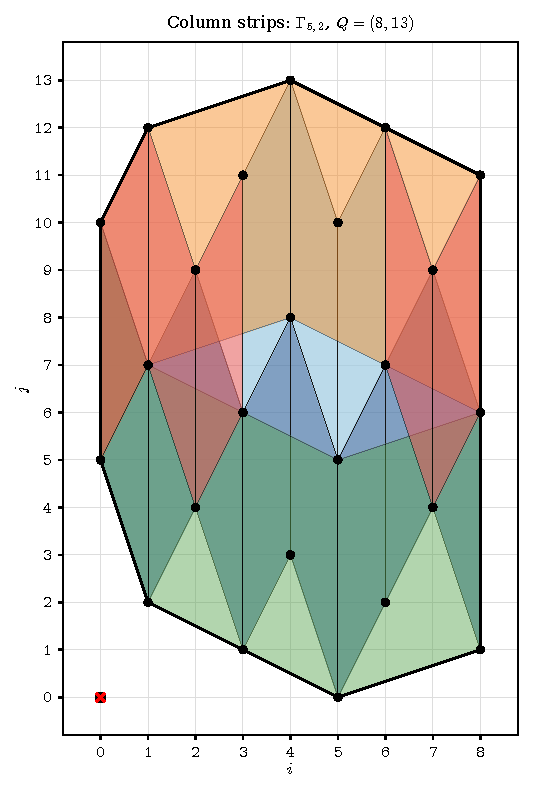
\includegraphics[width=.55\textwidth]{figures/fig06_columns.pdf}
\caption{Column-strip coverage for $d=5$, $s=2$ ($t=3$), $Q=(8,13)$. Blue: stacked translates by $(0,d)$ over each unit slab; red: mismatch triangles where adjacent columns have different heights $K_i\ne K_{i+1}$; green: lower sliver cells (translates of lower-hull pieces by $(0,d)$); purple: upper sliver cells (translates of upper-hull pieces by $(0,-d)$).}\label{fig:columns}
\par\smallskip\noindent\figdesc{A tall rectangle $[0,8]\times[0,13]$ with the hull of the lattice points drawn and tiled almost entirely by blue parallelograms stacked vertically in each unit-wide column, with a few red triangles where neighbouring columns end at different heights, and green and purple strips along the lower and upper boundary.}
\end{figure}

\begin{proof}[Proof of Theorem~\ref{thm:large}]
\emph{Column cells.} Fix a slab $i\le x\le i+1$, $0\le i<Q_1$, and put $\delta=b_{i+1}-b_i$ and $m=\min(K_i,K_{i+1})\ge1$. For $0\le k<m$ the parallelogram
\[
  E_{i,k}=P\bigl(B_i+k(0,d);\ (1,\delta),\ (0,d)\bigr)
\]
has corners $B_i+k(0,d)$, $B_i+(k+1)(0,d)$ in column $i$ and $B_{i+1}+k(0,d)$, $B_{i+1}+(k+1)(0,d)$ in column $i+1$; these are points of $F_Q$ by Lemma~\ref{lem:columns}(1) since $k+1\le m\le K_i,K_{i+1}$. The generators are Graver (Lemma~\ref{lem:columns}(2)) and independent ($\cross=d$). Let $P_B$ be the piecewise linear function with $P_B(i)=b_i$. The cells $E_{i,0},\dots,E_{i,m-1}$ stack and cover $\{P_B\le y\le P_B+md\}$ over the slab.

\emph{Mismatch triangle.} Let $P_T$ be the piecewise linear function with $P_T(i)=\tau_i$ (the ordinate of $T_i$). If $K_i=K_{i+1}$ then $P_T=P_B+md$ on the slab and nothing more is needed. If $K_i\ne K_{i+1}$ then by Lemma~\ref{lem:columns}(3) they differ by exactly $1$, and $P_T-(P_B+md)$ is the linear function equal to $0$ at the end with the smaller $K$ and to $d$ at the other end; the region between is a triangle with vertices $T_i$, $T_{i+1}$ and the point $T_j-(0,d)$ of the taller column $j\in\{i,i+1\}$. Consider
\[
  G_i=P\bigl(T_i;\ T_{i+1}-T_i,\ (0,-d)\bigr),
\]
with corners $T_i,\ T_{i+1},\ T_i-(0,d),\ T_{i+1}-(0,d)$. All four are in $F_Q$ because $K_i,K_{i+1}\ge1$, the generator $T_{i+1}-T_i$ is Graver by Lemma~\ref{lem:columns}(4), and $\cross\bigl(T_{i+1}-T_i,(0,-d)\bigr)=-d$. The triangle is contained in $G_i$, since its three vertices are corners of $G_i$.

\emph{Hull pieces.} Let $l(x)$ and $r(x)$ be the lower and upper ordinates of $H_Q$ at the abscissa $x\in[0,Q_1]$. Since $H_Q$ is a convex polygon with all vertices in $F_Q$, and every column contains at least two points, a vertex of $H_Q$ that is not the lowest point of its column cannot lie on the lower boundary (the lattice point of $F_Q$ just below it is in $H_Q$), and similarly for the upper boundary. Thus every lattice point of $\Gamma$ on the lower boundary of $H_Q$ is a column bottom $B_i$, and every lattice point on the upper boundary is a column top $T_i$. Let $p,p'$ be consecutive boundary lattice points on the lower boundary, with $p_1<p'_1$; they are column bottoms and $p'-p$ is Graver by the boundary Lemma~\ref{lem:reflection}. Put
\[
  S^-(p,p')=P\bigl(p;\ p'-p,\ (0,d)\bigr).
\]
Its corners $p+(0,d)$, $p'+(0,d)$ are in the box because $p_2,p'_2\le d$ and $Q_2\ge2d$, and they are nonzero; so it is admissible ($p'-p$ is not vertical, hence independent of $(0,d)$). It covers $\{l\le y\le l+d\}$ over $[p_1,p'_1]$. Since $0\le l\le P_B\le d$ we have $P_B\le l+d$ and so this cell covers the \emph{lower sliver} $\{l\le y\le P_B\}$. Similarly for consecutive boundary lattice points $p,p'$ on the upper boundary, with $p_1<p'_1$, which are column tops with ordinates $>Q_2-d$, put $S^+(p,p')=P(p;p'-p,(0,-d))$; its corners $p-(0,d)$, $p'-(0,d)$ have ordinates $>Q_2-2d\ge0$ and are in $F_Q$; it covers $\{r-d\le y\le r\}$. Since $P_T\ge Q_2-d\ge r-d$, it covers the \emph{upper sliver} $\{P_T\le y\le r\}$.

\emph{Conclusion.} At every abscissa $x\in[0,Q_1]$ the vertical slice $[l(x),r(x)]$ of $H_Q$ is the union of the lower sliver $[l,P_B]$, the stack $[P_B,P_B+md]$, the mismatch triangle $[P_B+md,P_T]$ and the upper sliver $[P_T,r]$, because $l\le P_B\le P_B+md\le P_T\le r$. Each is covered by an admissible cell. Hence $H_Q\subseteq U_Q$.
\end{proof}

\begin{remark}
The hypothesis $\max(Q_1,Q_2)\ge2d$ is used in four places: the existence of two points in each column, and the three box containments for the shifted cells ($p+(0,d)$ for bottoms, $p-(0,d)$ for tops, and the mismatch cell $G_i$). It is not available in the small-box regime; there the columns may contain a single point, which is why a different mechanism (Sections~\ref{sec:exceptional}--\ref{sec:cap}) is needed.
\end{remark}

%% -------------------------------------------------------------------
\section{An arithmetic inequality for Pareto-minimal points}\label{sec:pareto}

From here on we write $a=d-s$ and $c=d-t$. Note that $ac\equiv st\equiv1\pmod d$.

\begin{definition}[Pareto-minimal point]
A point $M=(x,y)\in\Gamma$ with $0<x,y<d$ is \emph{Pareto-minimal} if $\Gamma\cap([0,x]\times[0,y])=\{0,M\}$.
\end{definition}

A Pareto-minimal point has no other nonzero lattice point weakly below and to the left of it. Every Pareto-minimal point is a Graver vector: a vector $h\in\Gamma$ with $h\conf M$ satisfies $0\le h_1\le x$, $0\le h_2\le y$ (since $M$ has positive coordinates, conformality means the same signs), so $h\in\{0,M\}$.

\begin{lemma}[Arithmetic inequality; GEO-I G12-T1]\label{lem:arith}
Let $s\not\equiv-1\pmod d$ (so that $a,c\ge2$; this includes all nonspecial classes), and let $M=(x,y)$ be Pareto-minimal. Then
\[
  \boxed{\ \max\{\,y+a\,x,\ x+c\,y\,\}\ \ge\ xy.\ }
\]
\end{lemma}
\begin{proof}
Both $y+ax$ and $x+cy$ are positive multiples of $d$: modulo $d$, $y+ax\equiv y-sx\equiv0$ and $x+cy\equiv x-ty\equiv x-tsx\equiv0$. Suppose, to reach a contradiction, that
\[
  y+ax<xy\quad\text{and}\quad x+cy<xy.
\]
\emph{The case $x=1$ (or $y=1$).} If $x=1$ the first inequality reads $y+a<y$, which is false. If $y=1$ the second reads $x+c<x$, which is false. So $x,y\ge2$.

\emph{Consequences of the inequalities.} From $y+ax<xy$ we get $ax<y(x-1)<yx$, so $a<y$. From $x+cy<xy$ we get $c<x$.

\emph{Step 1: $y+ax=d$.} Write $y+ax=bd$ with $b\ge1$. Suppose $b\ge2$. Put $r=\lceil(d-y)/a\rceil$ and $R=(x-r,\ y-d+ar)$. Then:
\begin{itemize}
\item $R\in\Gamma$: $R=M-r(1,s-d)-(0,d)$ and $(1,s-d),(0,d)\in\Gamma$.
\item $r\ge1$ since $y<d$, and $r\le x$ since $y+ax=bd>d$ gives $(d-y)/a<x$; hence $0\le R_1\le x-1$.
\item $R_2\ge0$ because $ar\ge d-y$; and $R_2\le y$ because $ar<(d-y)+a$ gives $R_2<a<y$.
\item $R\ne0$: $R_2+aR_1=y-d+ar+a(x-r)=y+ax-d=(b-1)d>0$.
\end{itemize}
Thus $R$ is a nonzero lattice point of $[0,x]\times[0,y]$ different from $M$ (as $R_1<x$), contradicting Pareto-minimality. Therefore $b=1$.

\emph{Step 2: $x+cy=d$.} Apply Step 1 to the transposed point $(y,x)$ in $\Gamma_{d,t}$, where the roles of $a$ and $c$ are exchanged.

\emph{Step 3: contradiction.} Since $a,c\ge2$, $ac\ge4>1$ and $ac\equiv1\pmod d$, we can write $ac-1=md$ with $m\ge1$. From $y=d-ax$ and $x+cy=d$:
\[
  x+c(d-ax)=d\ \Longrightarrow\ x(ac-1)=d(c-1)\ \Longrightarrow\ mx=c-1.
\]
So $x\le c-1<c$, contradicting $c<x$.
\end{proof}

\begin{remark}[Role of the inequality]
The two numbers $y+ax$ and $x+cy$ are the determinants $\cross(g,M)$ for $g=(1,-a)$ and $g=(c,-1)$ respectively. The lemma says that for at least one of the two Graver vectors $g$ the parallelogram spanned by $g$ and $M$ has area at least $xy$, the area of the rectangle $[0,x]\times[0,y]$. This is exactly the condition under which the bottom cell of Section~\ref{sec:cellfamily} contains the triangle $\Delta_B$.
\end{remark}

\begin{figure}[ht]
\centering
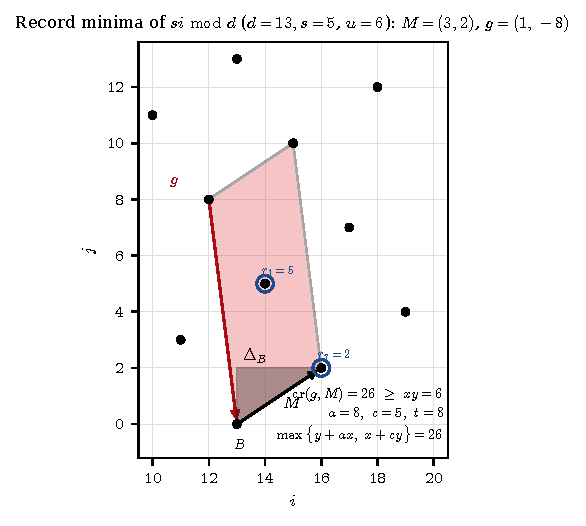
\includegraphics[width=.9\textwidth]{figures/fig07_records.pdf}
\caption{Record minima of $si\bmod d$ and the bottom cell: $d=13$, $s=5$ ($t=8$, $a=8$, $c=5$), $u=6$. The circled points are the records $r_i$; $M=(x,y)$ is the last (smallest) record; $g$ is the chosen Graver vector for which $\cross(g,M)\ge xy$; the shaded parallelogram is $P(B-g;g,M)$ and the dark triangle is $\Delta_B$.}\label{fig:records}
\par\smallskip\noindent\figdesc{A plot of the lattice points of $\Gamma_{13,5}$ to the right of $B=(13,0)$, with the record minima circled in blue and labelled by their ordinates; an arrow $M$ from $B$ to the last record, an arrow $g$ ending at $B$, and a shaded parallelogram with a dark triangle $\Delta_B$ at its right. The lower right corner states the numerical comparison $\cross(g,M)\ge xy$.}
\end{figure}

%% -------------------------------------------------------------------
\section{The boundary Graver reflection theorem}\label{sec:reflection}

\begin{lemma}[Axis pairs are never consecutive]\label{lem:axis-pair}
Let $Q_1,Q_2\ge d$ and let $k,\ell\ge1$ be integers with $kd\le Q_1$ and $\ell d\le Q_2$. Then $(kd,0)$ and $(0,\ell d)$ are not consecutive lattice points on $\partial H_Q$. In particular $B$ and $A$ are never consecutive.
\end{lemma}
\begin{proof}
Suppose they are consecutive. Then the segment between them lies in $\partial H_Q$, and its supporting line $x/(kd)+y/(\ell d)=1$ has $H_Q$ on one side. The point $(kd,\ell d)\in\Gamma$ lies in the box and is nonzero, hence belongs to $F_Q\subseteq H_Q$; the left-hand side equals $2>1$ there. So $x/(kd)+y/(\ell d)\ge1$ on $H_Q$. The points $(d,0)$ and $(0,d)$ are in $F_Q$ since $Q\ge(d,d)$, which gives $1/k\ge1$ and $1/\ell\ge1$, so $k=\ell=1$. Now $(1,s)\in F_Q$ gives $(1+s)/d\ge1$, so $s=d-1$. But then $(1,d-1)$ lies on the open segment between $A$ and $B$, and is a lattice point of $\Gamma$ on $\partial H_Q$ strictly between them, contradicting consecutiveness.
\end{proof}

\begin{lemma}[Boundary Graver lemma; GEO-I G12-T2]\label{lem:reflection}
Let $d\ge2$, $s$ any unit, and $Q_1,Q_2\ge d$ (with no upper bound on $Q$). Let $w,w'$ be two consecutive points of $\Gamma$ on the boundary of $H_Q$, where \emph{all} lattice points of $\Gamma$ on the boundary, including collinear ones, are listed. Then $w'-w$ is a Graver vector.
\end{lemma}

Note that $0\notin H_Q$ (the origin is an extreme point of the quadrant containing $F_Q$, and $F_Q\not\ni0$), so every lattice point on $\partial H_Q$ lies in $F_Q$. Consecutive boundary lattice points lie on a common side of the polygon $H_Q$, since the vertices of $H_Q$ are lattice points.

\begin{proof}
Put $e=w'-w\ne0$ and suppose for contradiction that there is $h\in\Gamma\setminus\{0,e\}$ with $h\conf e$. Put $h'=e-h$; then $h'\in\Gamma\setminus\{0,e\}$ and $h'\conf e$ as well. Let $p=w+h$ and $p'=w'-h=w+h'$. Both lie in the axis-parallel rectangle spanned by $w$ and $w'$, which is contained in the box. They satisfy
\[
  p+p'=w+w'.
\]

\emph{Step 1: $p$ and $p'$ are nonzero.} Suppose $p=0$ (the case $p'=0$ is the same with $w$ and $w'$ exchanged). In each coordinate $i$ with $w_i>0$, $w_i+h_i=0$ gives $h_i=-w_i<0$, so $e_i<0$ by conformality and $|e_i|\ge|h_i|=w_i$, whence $w'_i=w_i+e_i\le0$, i.e. $w'_i=0$. In a coordinate with $w_i=0$ we have $h_i=0$. Since $w\ne0$ some coordinate of $w$ is positive; if both were positive then $w'=0$, impossible. So exactly one coordinate of $w$ is positive; since $w'\ne0$ the other coordinate of $w'$ is positive. As $w,w'\in\Gamma$ and a point of $\Gamma$ on an axis has coordinate divisible by $d$,
\[
  \{w,w'\}=\{(kd,0),\ (0,\ell d)\}\qquad\text{for some integers }k,\ell\ge1.
\]
Both points lie in the box, since $w,w'$ do. This is impossible by Lemma~\ref{lem:axis-pair}, because $w$ and $w'$ are consecutive. So $p,p'\ne0$, hence $p,p'\in F_Q$.

\emph{Step 2: reflection.} Let $\varphi$ be an affine function with $\varphi=0$ on the line through $[w,w']$ and $\varphi\ge0$ on $H_Q$ (a supporting functional). Since $\varphi$ is affine and $p+p'=w+w'$,
\[
  \varphi(p)+\varphi(p')=\varphi(w)+\varphi(w')=0.
\]
Both terms are $\ge0$ because $p,p'\in F_Q\subseteq H_Q$. Hence $\varphi(p)=\varphi(p')=0$: both lie on the supporting line, which meets $H_Q$ in the side containing $[w,w']$.

\emph{Step 3: contradiction.} The vector $h=p-w$ is parallel to $e$, so $h=\theta e$ for some $\theta\in\R$. Conformality $h\conf e$ gives $0\le\theta\le1$, and $h\ne0,e$ gives $0<\theta<1$. Then $p=w+\theta e$ is a lattice point of $\Gamma$ on the open segment between the consecutive boundary lattice points $w$ and $w'$, a contradiction. Therefore no such $h$ exists and $e$ is Graver.
\end{proof}

\begin{remark}[Scope: no upper bound on the box]
The statement and proof hold for \emph{every} box with $Q_1,Q_2\ge d$. The earlier source version of this lemma (GEO-I v012, G12-T2) concluded in Step~1 that $\{w,w'\}=\{B,A\}$ directly, which is only correct when the axis points of $F_Q$ are $A$ and $B$, that is, for $Q<2d$. The argument above does not need this: it handles the axis pairs $(kd,0),(0,\ell d)$ with arbitrary $k,\ell$ by the support argument. This was the correction recorded as D4 in Appendix~\ref{app:corrections}.
\end{remark}

\begin{corollary}[Legitimacy of the cell generators]\label{cor:generators}
Every edge $w\to w'$ of the boundary of $H_Q$ between consecutive lattice points gives a Graver generator $w'-w$ for admissible parallelograms $P(w;w'-w,g)$ and admissible segments, for every Graver $g$ and every translate with corners in $F_Q$. In particular the steps of the lower-left chain (Lemma~\ref{lem:chain0}), the steps of the outer chain $\Omega$ (Section~\ref{sec:chain}) and the hull pieces in the large-box proof are Graver vectors.
\end{corollary}
